% !TeX spellcheck = it_IT
\newpage
\section{Logica del prim'ordine}
Il problema principale della logica proposizionale è che non ha la potenza espressiva per descrivere un ambiente con molti oggetti in modo conciso. Nella logica del prim'ordine abbiamo assunzioni più ricche riguardo la natura della realtà: \textit{oggetti}, \textit{relazioni}, \textit{proprietà}.\\

\subsection{Concettualizzazione}
Il primo passo è quello di decidere quali sono le cose di cui vogliamo parlare, dobbiamo quindi definire gli \textbf{oggetti}, che possono essere identificati da \textit{simboli} o da \textit{funzioni} che li mettono in relazione con altri oggetti. L'insieme degli oggetti rilevanti costituiscono il \textbf{dominio del discorso}, che potrebbe anche essere infinito.\\
Ci sono poi le \textbf{relazioni}, le \textbf{proprietà} (unarie) e le funzioni (biettive).

\begin{example}[Mondo dei blocchi]
	Siamo in un mondo di blocchi, che ad esempio può essere strutturato nel seguente modo:
	\begin{center}
		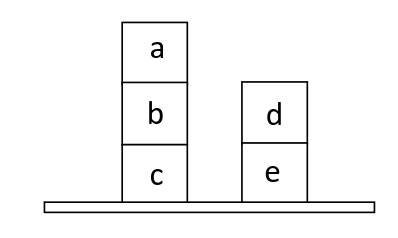
\includegraphics[scale=0.2]{block_world.png}
	\end{center}
	Per prima cosa definiamo il \textit{dominio} composto dai blocchi presenti:
	\begin{equation*}
		\{a,b,c,d,e\}
	\end{equation*}
	Poi individuiamo le \textit{funzioni} rilevanti ad identificare gli oggetti, nel nostro caso solo quella che, dato un blocco, identifica quello che ci sta sopra:
	\begin{equation*}
		Hat(b)=a
	\end{equation*}
	Infine abbiamo le \textit{relazioni}:
	\begin{gather*}
		On=\{<a,b>,<b,c>,<d,e>\} \\
		Clear=\{a,d\}\\
		Table=\{c,e\}\\
		Block=\{a,b,c,d,e\}
	\end{gather*}
	Riassumiamo la nostra \textbf{concettualizzazione} come la seguente tupla composta da \textit{dominio}, \textit{funzioni} e \textit{relazioni}:
	\begin{equation*}
		<\{a,b,c,d,e\}, \{Hat\}, \{On, Clear, Table, Block\}>
	\end{equation*}
\end{example}

\subsection{Sintassi}
\subsubsection{Simboli}
Gli elementi sintattici di base sono i simboli usati per indicare oggetti, relazioni e funzioni. Ne abbiamo di tre tipi:
\begin{itemize}
	\item \textbf{Simboli di costante}: rappresentano gli oggetti
	\item \textbf{Simboli di predicato}: rappresentano le relazioni
	\item \textbf{Simboli di funzione}: rappresentano le funzioni
\end{itemize}
Ogni simbolo degli ultimi due tipi ha una specifica \textbf{arità}, che ne indica il numero di \textit{argomenti}.\\
Quando gli oggetti non sono specificati, usiamo le \textbf{variabili}, che ci consentono di formulare predicati che possono essere veri o falsi a seconda di che valore assegnamo.

\subsubsection{Termini}
Un termine è un'espressione logica che si riferisce ad un oggetto. Ha la seguente sintassi:
\begin{equation*}
	Termine \to Costante \vert Variabile \vert Funzione(Termine, \ldots)
\end{equation*}
\begin{example}
	Alcuni esempi di termini ben formati:
	\begin{gather*}
		f(x,y) \quad +(2,3) \quad Padre-di(Giovanni) \\
		x,A,B,2 \quad Prezzo(Banane) \quad Hat(A)
	\end{gather*}
\end{example}

Il simbolo di \textbf{uguaglianza} si usa per dire che due termini fanno \textit{riferimento} allo stesso oggetto:
\begin{equation*}
	\exists x,y \quad Fratello(x, Riccardo)\land Fratello(y, Riccardo) \land \neg (x=y)
\end{equation*}

\subsubsection{Formule}
Una formula \textbf{atomica} è l'espressione più semplice e \textit{indivisibile} che afferma una relazione tra oggetti del dominio. È composta da un \textit{predicato} seguito da una \textit{lista di termini} che corrispondono alla sua arità. Le formule atomiche non contengono quantificatori, connettivi logici o altre formule come componenti. Ha la seguente sintassi:
\begin{align*}
	\text{Formula-atomica} \rightarrow & True \vert False \vert \\
	& \text{Termine} = \text{Termine } \vert\\
	& \text{Predicato}(\text{Termine}, \ldots)
\end{align*}
Ci sono poi le formule \textbf{complesse}, nelle quali possiamo usare \textit{connettivi logici} e \textit{quantificatori}. Hanno la seguente sintassi:
\begin{align*}
	\text{Formula} \rightarrow & \text{Formula-atomica } \vert \\
	& \text{Formula} \quad \text{Connettivo} \quad \text{Formula } \vert \\
	& \text{Quantificatore} \quad \text{Variabile} \quad \text{Formula } \vert \\
	& \neg \text{Formula } \vert (\text{Formula})
\end{align*}

\begin{example}
	Alcune formule \textit{atomiche} ben formate:
	\begin{gather*}
		Ama(Giorgio, Lucia) \quad On(A,B) \quad Madre-di(Luigi) = Silvana \\
		Amico(Padre-di(Giorgio), Padre-di(Elena)) \quad +(2,3)=5 \quad x=5
	\end{gather*}
	Alcune formule \textit{complesse} ben formate:
	\begin{gather*}
		On(A,B) \land On(B,C) \\
		Studia(Paolo) \Rightarrow Promosso(Paolo)
	\end{gather*}
\end{example}

\subsubsection{Quantificatori}
Esistono due tipi di quantificatori:
\begin{itemize}
	\item \textbf{Universale}: la relazione si applica a tutti gli elementi del dominio (e.g. $\forall x \quad Ama(x, Gelato)$)\\
	\item \textbf{Esistenziale}: la relazione si applica ad almeno un elemento del dominio (e.g. $\exists x \quad Mela(x) \land Rossa(x)$)
\end{itemize}
\begin{note}
	L'ordine dei quantificatori è importante.
\end{note}
Ogni quantificatore ha un suo \textbf{scope}, ad esempio nel seguente predicato
\begin{equation*}
	\forall x (\exists y \quad Ama(x,y))
\end{equation*}
$\exists y$ ha come scope $Ama(x,y)$ mentre $\forall x$ ha come scope $(\exists y \quad Ama(x,y))$.
\subsubsection{Linguaggio}
Il linguaggio della logica del prim'ordine è descritto dal seguente vocabolario:
\begin{align*}
	&\text{Connettivo} \rightarrow \land \vert \lor \vert \neg \vert \Rightarrow\vert\Leftrightarrow\vert\Leftarrow \\
	&\text{Quantificatore}\rightarrow\forall\vert\exists\\
	&\text{Variabile}\rightarrow x\vert y \vert \ldots \vert a \vert \ldots \vert s \vert \ldots\\
	&\text{Costante} \rightarrow A \vert B \vert \ldots \vert Mario \vert Pippo \vert \ldots \vert 1 \vert \ldots\\
	&\text{Funzione} \rightarrow Hat \vert Padre-di \vert + \vert - \vert \ldots\\
	&\text{Predicato} \rightarrow On \vert Clear \vert \geq \vert < \vert \ldots
\end{align*}
Quando utilizziamo le variabili nell'ambito dei quantificatori sono definite \textbf{legate}, altrimenti sono \textbf{libere}.

\begin{definition}[Formula chiusa]
	Una formula che non contiene occorrenze di variabili libere.
\end{definition}
\begin{definition}[Formula aperta]
	Una formula che contiene occorrenze di variabili libere.
\end{definition}
\begin{definition}[Formula ground]
	Una formula che non contiene variabili.
\end{definition}

\begin{observation}[Precedenza]
	Nel linguaggio della logica del prim'ordine è importante la precedenza tra gli operatori logici. Ad esempio:
	\begin{align*}
		\forall x \quad Persona(x) \Rightarrow Sesso(x)=M \lor Sesso(x)=F \lor Sesso(x)=NB \\
		\lor  Sesso(x)=GQ \lor Sesso(x)=GF \lor Sesso(x)=A
	\end{align*}
	deve essere interpretata come:
	\begin{align*}
		\forall x \quad (Persona(x) \Rightarrow ((Sesso(x)=M) \lor (Sesso(x)=F) \lor (Sesso(x)=NB) \\
		\lor (Sesso(x)=GQ) \lor (Sesso(x)=GF) \lor (Sesso(x)=A)))
	\end{align*}
\end{observation}

\subsection{Semantica}
La logica del prim'ordine usa una semantica di tipo \textbf{dichiarativo}, che consiste nello stabilire una corrispondenza tra:
\begin{itemize}
	\item I \textit{termini} del linguaggio e gli \textit{oggetti} del mondo
	\item Le \textit{formule chiuse} e i \textit{valori di verità}
\end{itemize}

\subsubsection{Componenti}
Le componenti principali della semantica sono:
\begin{itemize}
	\item \textbf{Universo} del discorso: un insieme non vuoto di elementi che rappresenta l'insieme di tutti gli \textit{oggetti} che si prendono in considerazione
	\item \textbf{Assegnazione di valori}:
	\begin{itemize}
		\item Alle \textit{costanti} si assegna un elemento specifico dell'universo
		\item Alle \textit{variabili} si possono assegnare elementi dell'universo attraverso una \textit{funzione}
		\item Alle \textit{funzioni} si assegna una mappatura da una sequenza di elementi dell'universo ad un singolo elemento dell'universo (rispettando la sua \textit{arità})
		\item Ai \textit{predicati} si assegna una relazione sull'universo (rispettando la sua \textit{arità})
	\end{itemize}
	\item \textbf{Verità di formule}:
	\begin{itemize}
		\item Una formula \textit{atomica} è vera se l'interpretazione assegna ai suoi termini una sequenza che rientra nella relazione specificata dal predicato
		\item Una formula \textit{complessa} viene valutata sulla  base dei suoi componenti usando il significato dei \textit{connettori logici} e dei \textit{quantificatori}
	\end{itemize}
\end{itemize}

\subsubsection{Interpretazione}
Una interpretazione $I$ stabilisce una \textit{corrispondenza} tra elementi atomici del linguaggio ed elementi della concettualizzazione. Interpreta:
\begin{itemize}
	\item I simboli di \textit{costante} come elementi del dominio $D$
	\item I simboli di \textit{funzione} come funzioni da n-uple di $D$ in $D$
	\item I simboli di \textit{predicato} come insiemi di n-unple (relazioni)
\end{itemize}

\begin{example}
	Partiamo da un'altra versione del mondo dei blocchi:
	\begin{center}
		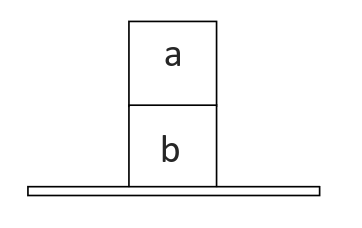
\includegraphics[scale=0.2]{block_world_2.png}
	\end{center}
	concettualizzato come segue:
	\begin{align*}
		On(A,B) \\
		Clear(A) \\
		Table(B)
	\end{align*}
	Una possibile interpretazione è la seguente:
	\begin{align*}
		&I(A)=a \quad I(B)=b \\
		&I(On)=\{<a,b>\}\\
		&I(Clear)=\{a\}\\
		&I(Table)=\{b\}
	\end{align*}
	ma lo è anche:
	\begin{align*}
		&I(A)=a \quad I(B)=b \\
		&I(On)=\{<b,a>\}\\
		&I(Clear)=\{b\}\\
		&I(Table)=\{a\}
	\end{align*}
\end{example}
Quindi il significato di un termine o di una formula composta è determinato in funzione del significato dei suoi componenti.\\
Nel caso dei quantificatori:
\begin{itemize}
	\item \textbf{Universale}: $\forall x \: A(X)$ è vera se lo è per ciascun elemento del dominio di $A$. Se il dominio è \textit{finito} equivale ad una serie di $\land$. Data la forza del quantificatore universale, spesso si restringe il suo campo d'azione mediante $\Rightarrow$
	\item \textbf{Esistenziale}: $\exists x \: A(x)$ e vera se esiste almeno un elemento del dominio per cui $A$ è vera. Se il dominio è \textit{finito} equivale ad una serie di $\lor$. Data la debolezza del quantificatore esistenziale, di solito si usa con $\land$
\end{itemize}
Da questo possiamo derivare alcune proprietà che mettono in relazione i due quantificatori (a destra le proprietà della logica da cui sono derivate):
\begin{align*}
	&\forall x \: \neg P(x) \equiv \neg \exists x \: P(x) & \neg P \land \neg Q \equiv \neg (P \lor Q)\\
	&\neg \forall x \: P(x) \equiv \exists x \: \neg P(x)&\neg(P \land Q) \equiv \neg P \lor \neg Q \\
	&\forall x \: P(x) \equiv \neg \exists x \: \neg P(x) & P \land Q \equiv \neg(\neg P \lor \neg Q)\\
	&\neg \forall x \: \neg P(x) \equiv \exists x \: P(x) & P \lor Q \equiv \neg (\neg P \land \neg Q)
\end{align*}

\begin{note}
	La semantica standard, che segue la logica classica, è spesso molto prolissa anche per esprimere concetti molto semplici. Per combattere questo problema esiste la semantica dei \textbf{database} che parte dalle seguenti ipotesi per essere più concisa:
	\begin{itemize}
		\item \textit{Nomi unici}: simboli e oggetti distinti, ogni costante fa riferimento ad un oggetto distinto
		\item \textit{Mondo chiuso}: tutto ciò di cui non si sa che è vero, è falso, quindi le formule atomiche non conosciute come vere sono false
		\item \textit{Chiusura del dominio}: esistono solo gli oggetti di cui si parla. Ogni modello contiene un numero di elementi del dominio non superiore a quello degli elementi denominati dai simboli di costante
	\end{itemize}
\end{note}
\subsubsection{Knowledge Base}
Le interazioni con la Knowledge Base in logica del prim'ordine sono fatte sfruttando:
\begin{itemize}
	\item \textbf{Asserzioni}, ad esempio
	\begin{equation*}
		TELL(KB, Re(Giovanni))
	\end{equation*}
	\item \textbf{Interrogazioni}, ad esempio
	\begin{equation*}
		ASK(KB, Persona(Giovanni)) \longrightarrow Si
	\end{equation*}
\end{itemize}

\begin{example}[Wumpus World]
	Possiamo implementare l'esempio del Wumpus World (\ref{example:wumpus_world}) in FOL, descrivendo tutto in maniera più precisa. Alcuni casi:
	\begin{itemize}
		\item \textbf{Percezioni}: possiamo rappresentarle come un predicato binario $Percezione(5-upla, t)$
		\item \textbf{Regole} per le percezioni: ad esempio per lo scintillio
		\begin{gather*}
			\forall t,s,b,m,c \: Percezione( [s,b,Scintillio,m,c], t) \Rightarrow Scintillio(t)\\
			\forall t,s,b,m,c \: Percezione( [s,b,None,m,c], t) \Rightarrow \neg Scintillio(t)
		\end{gather*}
		\item Descrizione della \textbf{mappa}: ad esempio l'adiacenza di una casella
		\begin{equation*}
			\forall x,y,a,b \: Adiacente([x,y], [a,b]) \Leftrightarrow (x=a \land(y=b-1 \lor y=b+1)) \lor (y=b \land (x=a-1 \lor x=a+1))
		\end{equation*}
	\end{itemize}
\end{example}

\subsection{Inferenza}
Dobbiamo eliminare i quantificatori. Introduciamo prima il concetto di \textbf{sostituzione}: $A[x/g]$ è il risultato della sostituzione di $g$ per $x$ in $A$.
\subsubsection{Istanziazione}
L'instanziazione \textbf{universale} prevede di inferire tutte le formule ottenute sostituendo un termine \textit{ground} $g$ a una variabile quantificata universalmente $x$.
\begin{equation}
	\frac{\forall x \: A[x]}{A[x/g]}
\end{equation}
\begin{example}
	Data la proposizione
	\begin{equation*}
		\forall x \: Re(x) \land Avido(x) \Rightarrow Malvagio(x)
	\end{equation*}
	si possono ottenere:
	\begin{align*}
		&Re(Giovanni) \land Avido(Giovanni) \Rightarrow Malvagio(Giovanni)\\
		&Re(Padre(Giovanni))  \land Avido(Padre(Giovanni)) \Rightarrow Malvagio(Padre(Giovanni))
	\end{align*}
\end{example}
L'instanziazione \textbf{esistenziale} prevede di sostituire una variabile quantificata esistenzialmente con un unico nuovo simbolo costante.
\begin{equation}
	\frac{\exists x\: A[x]}{A[x/k]}
\end{equation}
Se $\exists$ non compare nello scope di $\forall$, $k$ è una costante nuova chiamata \textbf{costante di Skolem}, altrimenti va introdotta una \textbf{funzione di Skolem} nelle variabili quantificate universalmente. Alcuni esempi:
\begin{align*}
	&\exists x \: Padre(x, G) \longrightarrow Padre(K, G) \\
	&\forall x \exists y \: Padre(x,y) \longrightarrow \forall x \: Padre(x, p(x))
\end{align*}

\subsubsection{Grounding}
La riduzione a inferenza proposizionale è detta \textbf{grounding} e prevede i seguenti passaggi:
\begin{enumerate}
	\item Istanziazione universale
	\item Istanziazione esistenziale
	\item Sostituire le formule \textit{atomiche ground} con simboli proposizionali
\end{enumerate}
Il problema che rimane prima di poter applicare gli algoritmi già visti è che anche se le costanti sono in numero finito, in presenza di funzioni le istanze da creare sono infinite: ad esempio:
\begin{equation*}
	Giovanni, Padre(Giovanni), Padre(Padre(Giovanni)), \ldots
\end{equation*}

\begin{theorem}[Teorema di Herbrand]
	Se $KB \models \alpha$, allora c'è una dimostrazione che coinvolge solo un sotto-insieme finito della KB proposizionalizzata.
\end{theorem}
Per applicare il teorema appena enunciato si può procedere \textit{incrementalmente}:
\begin{enumerate}
	\item Creare le istanza con le costanti
	\item Creare le istanze con un solo livello di annidamento
	\item Procedere livello per livello finché non siamo in grado di costruire la dimostrazione proposizionale della formula che è conseguenza logica
\end{enumerate}
Se $KB\nvDash$ il processo non termina. Il problema è quindi \textbf{semidecidibile}.

\subsubsection{Forma a clausole}
Per estendere alla logica del prim'ordine il metodo di risoluzione dobbiamo prima estendergli anche la trasformazione in forma a clausole.\\
\textit{Costanti}, \textit{funzioni} e predicati sono come definiti ma escludendo formule atomiche del tipo $t_1 = t_2$. Definiamo quindi una clausola come un insieme di \textit{letterali} che rappresenta la loro disgiunzione:
\begin{align}
	& Clausola \rightarrow \{Letterale, \ldots, Letterale\}\\
	& Letterale \rightarrow Formula_atomica \: \vert \: \neg Formula_atomica
\end{align}
Una Knowledge Base è quindi un insieme di clausole.
\begin{theorem}
	Per ogni formula chiusa $\alpha$ del FOL è possibile trovare in maniera \textbf{effettiva}un insieme di clausole $FC(\alpha)$ che è soddisfacibile se e solo se $\alpha$ lo è. Allo stesso modo per l'insoddisfacibilità.
\end{theorem}
\begin{definition}[Effettivo]
	Esiste una procedura che può essere eseguita per trasformare la formula $\alpha$ in un insieme di clausole $FC(\alpha)$ tale che valga questo risultato.
\end{definition}

\begin{example}[Trasformazione in forma a clausole]
	Vediamo passo per passo il processo di trasformazione appena descritto applicato alla frase:
	\begin{equation*}
		\forall x(\forall y \: Animale(y) \Rightarrow Ama(x,y)) \Rightarrow (\exists y \: Ama(y,x))
	\end{equation*}
	\begin{enumerate}
		\item Eliminazione delle implicazioni
		\begin{align*}
			&\forall x \neg(\forall y \: Animale(y) \Rightarrow Ama(x,y)) \lor (\exists y \: Ama(y,x))\\
			&\forall x\neg(\forall y \: \neg Animale(y) \lor Ama(x,y)) \lor (\exists y \: Ama(y,x))
		\end{align*}
		\item Negazioni all'interno
		\begin{align*}
			&\forall x(\exists y \neg (\neg Animale(y) \lor Ama(x,y))) \lor (\exists y \: Ama(y,x)) \\
			&\forall x(\exists y (\neg\neg Animale(y) \land \neg Ama(x,y))) \lor (\exists y \: Ama(y,x))\\
			&\forall x(\exists y (Animale(y) \land \neg Ama(x,y))) \lor (\exists y \: Ama(y,x))
		\end{align*}
		\item Standardizzazione delle variabili: facciamo in modo che ogni quantificatore usi una variabile diversa
		\begin{equation*}
			\forall x(\exists y (Animale(y) \land \neg Ama(x,y))) \lor (\exists z \: Ama(z,x))
		\end{equation*}
		\item Skolemizzazione: eliminazione dei quantificatori esistenziali
		\begin{equation*}
			\forall x(Animale(F(x)) \land \neg Ama(x,F(x)))) \lor Ama(G(x),x)
		\end{equation*}
		\item Eliminazione quantificatori universali
		\begin{equation*}
			(Animale(F(x)) \land \neg Ama(x,F(x)))) \lor Ama(G(x),x)
		\end{equation*}
		\item Applico la forma normale congiuntiva
		\begin{equation*}
			(Animale(F(x)) \land Ama(G(x),x)) \land (\neg Ama(x, F(x)) \lor Ama(G(x), x))
		\end{equation*}
		\item Applico la notazione a clausole
		\begin{equation*}
			\{Animale(F(x)) \land Ama(G(x),x)\} \{\neg Ama(x, F(x)) \lor Ama(G(x), x)\}
		\end{equation*}
		\item Separazione delle variabili: clausole diverse devono avere variabili diverse
		\begin{equation*}
			\{Animale(F(x_1)) \land Ama(G(x_1),x_1)\} \{\neg Ama(x_2, F(x_2)) \lor Ama(G(x_2), x_2)\}
		\end{equation*}
	\end{enumerate}
\end{example}

\subsubsection{Unificazione}
\begin{definition}[Unificazione]
	Operazione mediante la quale si determina se due espressioni possono essere rese identiche mediante una sostituzione di termini a variabili. Il risultato è la \textbf{sostituzione} che rende le due espressioni identiche, detta \textbf{unificatore}, o FAIL, se le espressioni non sono unificabili.
\end{definition}
\begin{definition}[Sostituzione]
	Un insieme finito di associazioni tra variabili e termini in cui ogni variabile compare una sola volta sulla sinistra. Data una sostituzione $\sigma$ e un'espressione $A$, $A\sigma$ è un'istanza generata dalla sostituzione delle variabili con le corrispondenti espressioni.
\end{definition}
L'idea è di trovare l'unificatore più generale di tutti, il \textbf{Most General Unifier} (MGU).
\begin{theorem}
	L'unificatore più generale è unico, a parte i nomi delle variabili (l'ordine non conta).
\end{theorem}
L'algoritmo di unificazione prende in input due espressioni $p$ e $q$ e restituisce un MGU $\theta$ se esiste, altrimenti FAIL. Appena trova espressioni non unificabili fallisce. Una causa di fallimento sono sostituzioni circolari del tipo $x=f(x)$; questo controllo si chiama \textbf{occurr check}.

\begin{lstlisting}
	function Unify(x, y, t =vuoto) returns una sostituzione che rende x e y identici, o fallimento
		if t = fallimento then return fallimento
		else if x = y then return t // caso di successo
		else if Variabile?(x) then return Unify-Var(x, y, t)
		else if Variabile?(y) then return Unify-Var(y, x, t)
		else if Composta?(x) and Composta?(y) then // es. Op(F(A,B)) = F Args(F(A,B)=(A,B)
			return Unify(Args(x), Args(y), Unify(Op(x), Op(y), t))
		else if Lista?(x) and Lista?(y) then
			return Unify(Resto(x), Resto(y), Unify(Primo(x), Primo(y), t))
		else return fallimento
\end{lstlisting}

\begin{example}
	Vediamo un esempio di applicazione dell'algoritmo:
	\begin{enumerate}
		\item $UNIFY(P(A,y,z),P(x,B,z), \{\})$
		\item $UNIFY((A,y,z),(x,B,z), UNIFY(P,P,\{\}))$
		\item $UNIFY((A,y,z),(x,B,z),\{\})$
		\item $UNIFY((y,z),(B,z), UNIFY(A,x,\{\}))$
		\item $UNIFY((y,z),(B,z), UNIFY(x,A,\{\}))$
		\item $UNIFY((y,z),(B,z), UNIFY-VAR(x,A,\{\}))$
		\item $UNIFY((y,z),(B,z), \{x/A\})$
		\item $UNIFY(z),(z), \{y/B, x/A\})$
		\item $UNIFYz,z, \{y/B, x/A\})$
		\item $\{y/B, x/A\}$
	\end{enumerate}
\end{example}

\subsubsection{Risoluzione}
Data una clausola $\phi$ che contiene $A$, una clausola $\psi$ che contiene $\neg B$ e l'unificatore $\gamma=MGU(A,B)$ definiamo la \textbf{risolvente} come:
\begin{equation}
	((\phi \ \{A\}) \subset (\psi \ \{\neg B\}))\gamma
\end{equation}
\begin{example}
	Ad esempio:
	\begin{center}
		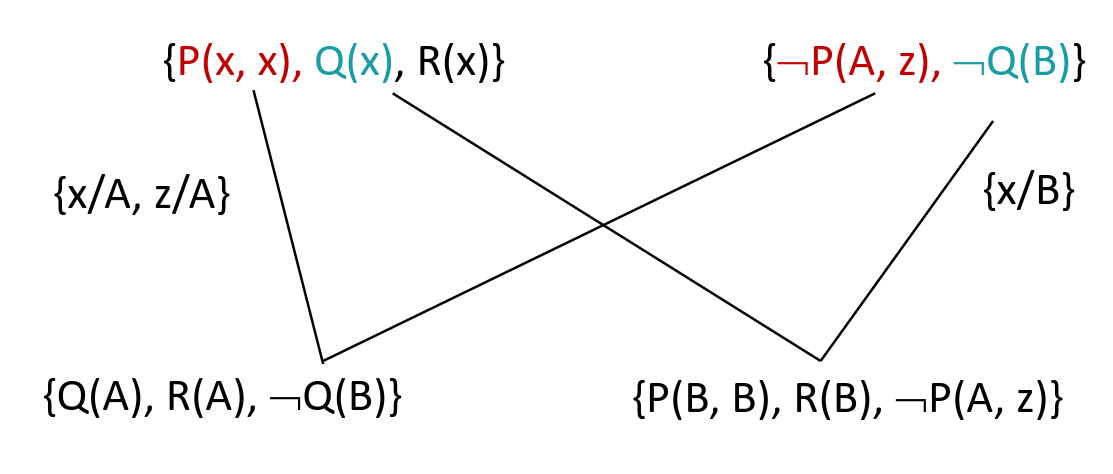
\includegraphics[scale=0.3]{fol_solution_graph.png}
	\end{center}
\end{example}

\begin{definition}[Fattori]
	Se un sottoinsieme dei letterali di una stessa clausola può essere unificato, allora la clausola ottenuta dopo tale unificazione si dice \textbf{fattore} delle clausole.
\end{definition}

\begin{observation}[Problema dei fattori]
	Ad esempio nel seguente caso le seguenti clausole dovrebbero produrre la clausola vuota, ma invece no.
	\begin{center}
		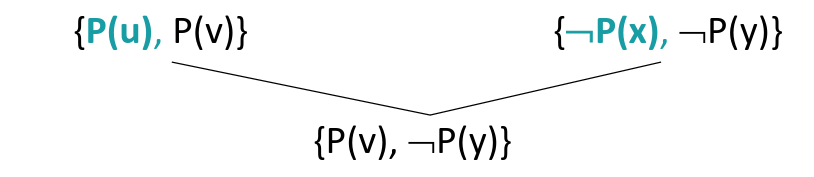
\includegraphics[scale=0.2]{fol_factors_problem.png}
	\end{center}
	È quindi necessario applicare il metodo di risoluzione ai fattori delle clausole.
	\begin{center}
		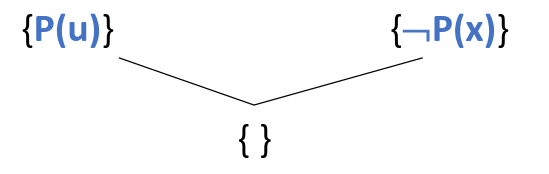
\includegraphics[scale=0.2]{fol_factors_problem_2.png}
	\end{center}
\end{observation}

La deduzione per risoluzione è \textbf{corretta} ma \textbf{non completa}. Per ottenere la completezza si può risolvere per \textbf{confutazione}.
\begin{example}
	Partiamo dalla seguente KB:
	\begin{align*}
		&\{P(A, J)\}\\
		& \{M(B, J)\}\\
		&\{\neg P(x,y), G(x,y)\}\\
		&\{\neg M(v,w), G(v,w)\}\\
		& \{\neg G(A, J)\}
	\end{align*}\\
	In questo caso il grafo è il seguente:
	\begin{center}
		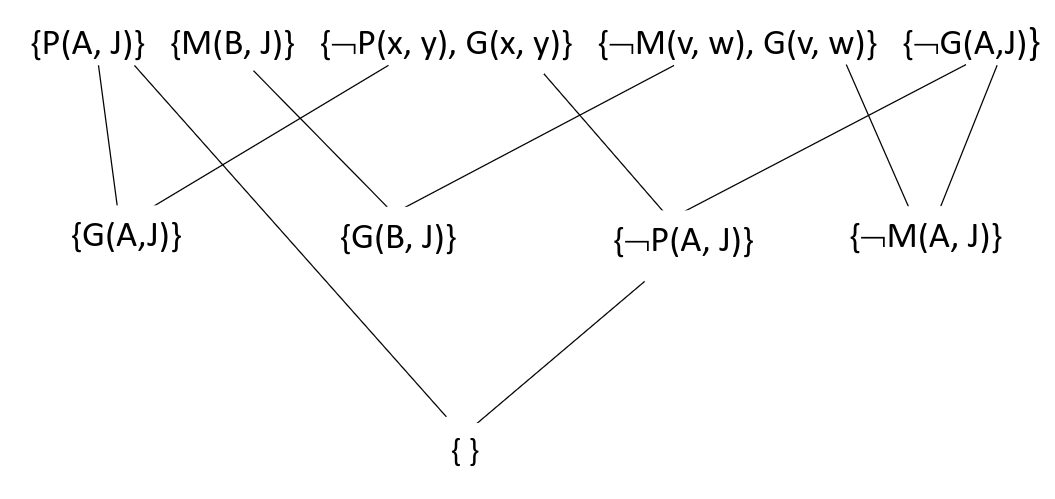
\includegraphics[scale=0.3]{fol_example_refutazione.png}
	\end{center}
\end{example}

\subsection{Programmazione logica}
\subsubsection{Clausola di Horn}
Una clausola di Horn è una \textbf{disgiunzione di letterali} che contiene al massimo un letterale positivo. È un modo potente ed efficiente per rappresentare conoscenze in logica del prim'ordine. È efficace in particolare per rappresentare regole e fatti in un sistema basato su regole.
\begin{equation}
	\{Q, \neg P_1, \ldots, \neg P_k\}\quad\quad k\geq 0
\end{equation} 
Possiamo quindi scrivere la knowledge base a regole come:
\begin{align*}
	P_1 \land \ldots \land P_k \Rightarrow Q \quad \text{(regola)}&& k>0 \\
	Q \quad\text{(fatto)}&& k=0
\end{align*}
Se la knowledge base contiene solo \textit{clausole Horn} definite, i meccanismi inferenziali sono più semplici (lineari per il caso proposizionale) senza dover rinunciare alla completezza.
\subsubsection{Inferenza}
I metodi usati nei sistemi basati su regole sono di due tipi:
\begin{itemize}
	\item Inferenza in \textbf{avanti}: si inizia con le \textit{premesse} e si procede verso le conclusioni partendo da un insieme di fatti noti e applicando le regole per dedurre nuove informazioni. Si continua fino a quando non si raggiunge un obiettivo o non si possono fare più inferenze
	\item Inferenza all'\textbf{indietro}: si inizia dalle \textit{conclusioni} e si lavora a ritroso per trovare le premesse che supportano la conclusione. Si verifica passo per passo se l'obiettivo corrente può essere dedotto dalle regole e se necessario si cerca all'indietro per dedurre o dimostrare i fatti richiesti dalle premesse.
\end{itemize}

\subsubsection{Programmazione}
I programmi logici sono KB costituiti di clausole Horn definite espressi come fatti e regole:
\begin{itemize}
	\item \textbf{Fatto}: un fatto è rappresentato da una singola clausola di Horn senza premesse
	\item \textbf{Regola}: sono implicazioni logiche che descrivono i come i fatti sono in relazione tra loro
\end{itemize}

\begin{note}[Convenzioni programmazione logica]
	Nella programmazione logica le \textbf{variabili} sono indicate con le lettere maiuscole e le \textbf{costanti} con quelle minuscole.
\end{note}
L'interpretazione può seguire due filosofie:
\begin{itemize}
	\item \textbf{Dichiarativa}: data la regola
	\begin{equation*}
		A :- B_1, \ldots, B_n 
	\end{equation*}
	$A$ è vero se sono veri $B_1, \ldots, B_n$ in accordo al significato logico dell'implicazione.
	\item \textbf{Procedurale}: sempre nel caso visto nel punto precedente, si considera la testa $A$ come una chiamata di procedura e il corpo come una serie di procedure da eseguire in sequenza
\end{itemize}

\begin{example}
	\label{example:pl}
	Ad esempio definiamo le seguenti regole, fatti e goal:
	\begin{align*}
		&genitore(X, Y) :- padre(X,Y).\\
		&genitore(X, Y) :- madre(X,Y).\\
		&antenato(X, Y) :- genitore(X,Y).\\
		&antenato(X, Y) :- genitore(X,Y), antenato(Z, Y).\\
		& padre(gio, mark).\\
		& padre(gio, luc).\\
		& madre(lia, gio).\\
		&:- antenato(lia, mark:)
	\end{align*}
\end{example}

\subsubsection{Risoluzione SLD}
La risoluzione di tipo \textbf{Selection Linear Definite-Clauses} è una strategia \textbf{ordinata} e \textbf{completa} per le clausole di Horn. A partire da un programma $P$ e un goal $G$ si costruisce l'albero di risoluzione, definito come:
\begin{itemize}
	\item Ogni \textbf{nodo} dell'albero corrisponde ad un goal
	\item La \textbf{radice} è $:- G_1, \ldots, G_k$, il goal di partenza
	\item Data la radice come nodo dell'albero, questo ha tanti \textbf{discendenti} quanti sono i fatti e le regole in $P$ la cui testa è unificabile con $G_1$
	\item I nodi che sono clausole vuote sono \textbf{successi}
	\item I nodi che non hanno successori sono \textbf{fallimenti}
\end{itemize}

\begin{example}
	Dato l'esempio \ref{example:pl}, il grafo di risoluzione è:
	\begin{center}
		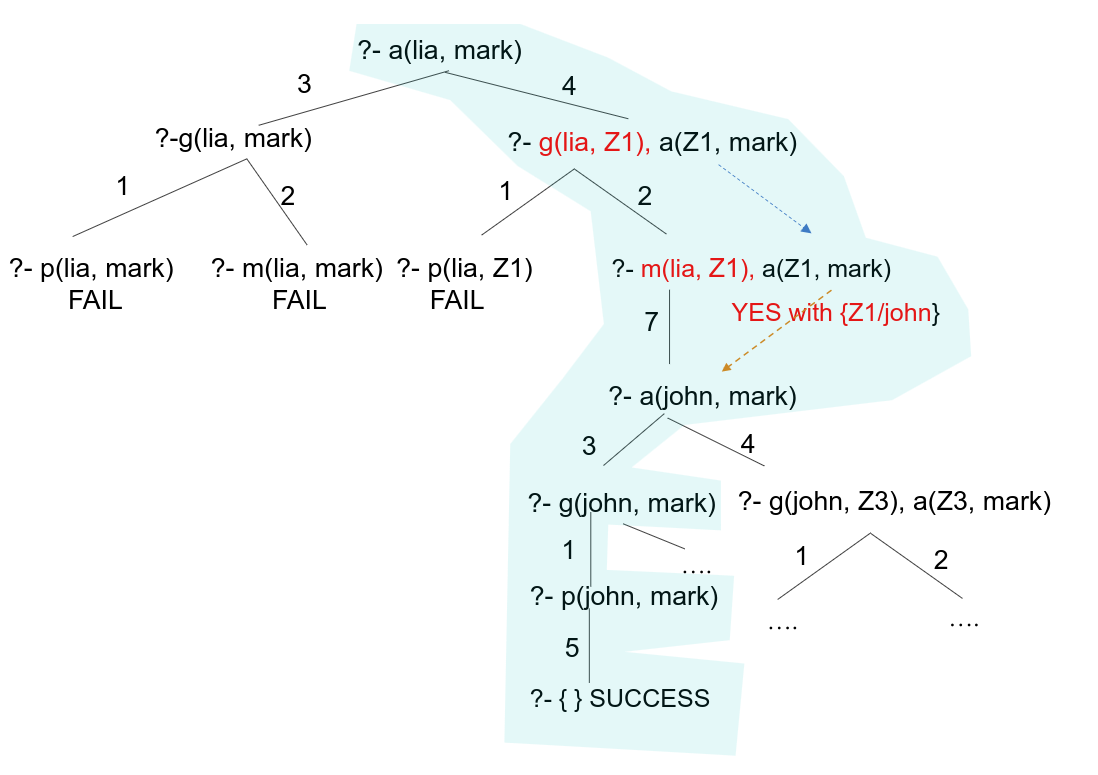
\includegraphics[scale=0.3]{pol_sdl.png}
	\end{center}
\end{example}

Questa strategia è \textbf{completa} per clausole di Horn definite.